\Section{preliminaries}{Preliminaries}

Our pruning technique works on Datalog, a general language which can be used to
express static analyses declaratively \cite{Whaley2007,bravenboer}.  Normally,
these analyses and their underlying abstractions are encoded by one monolithic Datalog program
which evaluates a query abstractly.
For us, it will be convenient to consider the
Datalog program, which evaluates a query concretely\footnote{We refer to this computation as ``concrete''
to contrast with abstract computation we will consider later,
but note that this ``concrete'' computation
could already contain some level of abstraction.
For example, the Datalog program might correspond to $\infty$-object-sensitivity
without abstraction and $k$-object-sensitivity with abstraction.
}, as distinct
from the abstraction, which is defined as a transformation on the input to
the Datalog program, and makes it evaluate the query abstractly.  This separation
allows us to make theoretical statements
comparing the behavior of the same Datalog program across different
abstractions.

We first define Datalog and the computation of a concrete query
(\refsec{datalog}).  Then, we focus on the abstraction (\refsec{abstractions}),
which interacts with the Datalog program by transforming the input tuples.
Throughout this section, we will use \reffig{graphExample} as a running example.

%%%%%%%%%%%%%%%%%%%%%%%%%%%%%%%%%%%%%%%%%%%%%%%%%%%%%%%%%%%%
\begin{figure}
\begin{center} {\bf Graph Example} \end{center}
{\bf Input relations}:
\[
\begin{array}{ll}
\edge(g,i,j) & \defn{edge from node $i$ to node $j$ in graph $g$} \\
\head(c,i)   & \defn{first element of array $c$ is $i$} \\
\ext(i,c,c') & \defn{$i$ prepended to $c$ yields $c'$: $c' = [i]+c$} \\
\end{array}
\]
{\bf Rules}:
\[
\begin{array}{lcl}
\path(g,[\initNode]). & \\
\path(g,c')           &\dlogUpdate& \path(g,c), \head(c,i), \\
                      &           & \edge(g, i, j), \ext(j, c, c'). \\
\common(g_1,g_2,i)    &\dlogUpdate& \path(g_1,c), \path(g_2,c), \head(c,i). \\
\end{array}
\]
{\bf Query tuple}: $\xo = \common(\Ga,\Gb,3)$. \\
\\
{\bf Constants}: $\sC = \{ \Ga, \Gb, 0, 1, 2, 3, \vec{0}, \vek{01}, \dots \}$.
\\
\\
%{\bf Abstraction}:
%$\alpha_k(c) = \{ c' : \text{$c$ and $c'$ have same length $k$ prefix}\}$
%\\
%\\
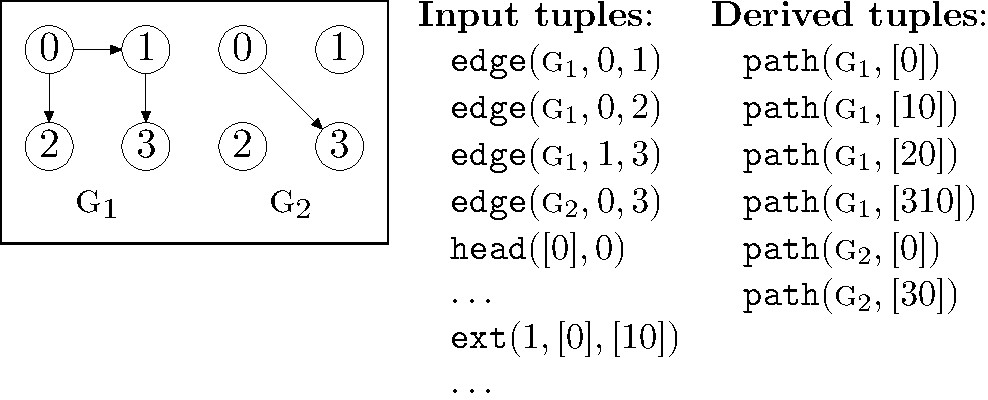
\includegraphics[scale=0.5]{figures/graphExample}
\caption{\label{fig:graphExample}
A simple example illustrating Datalog:
Suppose we have two graphs $\Ga$ and $\Gb$ defined on the same set of nodes $\{0,1,2,3\}$,
and we want to compute the query tuple $\common(\Ga,\Gb,3)$,
asking whether the two graphs have a common path from node $0$ to node $3$.
Given the input tuples encoding the graph,
the Datalog program computes a set of derived tuples from the rules.
In this case, the absence of $\common(\Ga,\Gb,3)$ from the derived tuples means the query is false (proven).
}
\end{figure}

%%%%%%%%%%%%%%%%%%%%%%%%%%%%%%
\Subsection{datalog}{Datalog}

A {\em Datalog program} consists of
a set of {\em constants} $\sC$ (e.g., $\initNode,\vec{03} \in \sC$),
a set of {\em variables} $\sV$ (e.g., $i, j \in \sV$), and
a set of {\em relations} $\sR$ (e.g., $\edge \in \sR$).

A {\em term} $t$ consists of a relation $t.r \in \sR$ and a list of arguments $t.\ba$,
where each argument $t.a_i$ is either a variable or a constant,
(that is, $t.a_i \in \sV \cup \sC$) for $i = 1, \dots, |t.\ba|$.
We will write a term in any of the following three equivalent ways:
\begin{align}
t \quad\equiv\quad t.r(t.\ba) \quad\equiv\quad t.r(t.a_1, \dots, t.a_{|t.\ba|}).
\end{align}
For example, $\ext(j,c,c')$ is a term.
We call a term whose arguments are all constants a {\em tuple}
(e.g., $\ext(\initNode, [\,], \vec{\initNode})$).
Note that the tuple includes the relation as well as the arguments.
We let $\xo$ denote a designated {\em query tuple} (e.g., $\common(\Ga,\Gb,3)$),
whose truth value we want to determine.

Let $\sZ$ denote the set of rules,
where each {\em rule} $z \in \sZ$ consists of a target term $z.t$ and a set of source terms $z.\bs$.
We write a rule if $z.t = t$ and $z.\bs = \{ s_1, \dots, s_k \}$ as
\begin{align}
t \dlogUpdate s_1, \dots, s_n.
\end{align}

An {\em assignment} is a function $f : \sV \mapsto \sC$ which maps variables to
constants.  To simplify notation later, we extend an assignment $f$ so that it
can be applied (i) to constants ($f(c) = c$ for $c \in \sC$), and (ii) to terms by
replacing the variables in the term with constants ($f(t) = t.r(f(t.a_1), \dots, f(t.a_{|t.\ba|}))$).

\begin{figure}[t]
%{\bf Notation:} \\
\[
\begin{array}{ll}
\xo                           & \defn{designated query tuple} \\
\sC                           & \defn{set of concrete values} \\
\bD(X)                        & \defn{derivations using input tuples $X$} \\
\bP(X) \subset X              & \defn{set of relevant input tuples} \\
\alpha : \sC \mapsto \sP(\sC) & \defn{abstraction, maps to equivalence class} \\
A_k \subset \sP(\sC)          & \defn{abstract input tuples after $k$ iterations} \\
\tilde A_k = \bP(A_k)         & \defn{relevant abstract input tuples} \\
\end{array}
\]
\caption{\label{fig:notation} Notation.}
\end{figure}

%%%%%%%%%%%%%%%%%%%%%%%%%%%%%%
%\Subsection{derivations}{Derivations}
\paragraph{Derivations}

A Datalog program takes a set of input tuples and derives new
tuples.  To formalize this computation, we define the notation of a derivation.

A {\em derivation} (of the query $\xo$) with respect to a set of input tuples
$X$ is a sequence $\bx = (x_1, \dots, x_n)$ such that
\begin{enumerate}
\item [(i)] for each $i = 1, \dots, n$, we have $x_i \in X$; or
there exists a set of indices $J$ such that $(J,i)$ satisfies the following conditions:
$j < i$ for each $j \in J$, and
there is a rule $z \in \sZ$ and an assignment $f$
such that $f(z.t) = x_i$ and
$\{ x_j : j \in J \} = \{ f(s) : s \in z.\bs \}$;
\item [(ii)] $x_n = \xo$; and
\item [(iii)] 
for each $j = 1, \dots, n\!-\!1$,
there exists $J$ such that $j \in J$ and an index $i$
such that $(J,i)$ satisfies the conditions in (i).
\end{enumerate}
Define $\bD(X)$ to be the set of all derivations with respect to the input tuples $X$.

% Explain
Condition (i) says that each tuple in a derivation
should either be given as an input tuple ($x_i \in X$)
or be the result of some rule $z \in \sZ$.
Condition (ii) says that $\xo$ was finally produced via some sequence of rule applications.
Condition (iii) says that in the derivation of $x_n$, every tuple is relevant for deriving $\xo$.
%As we will see later, this condition is important because it allow us to
%define the set of irrelevant tuples that can be pruned.

A Datalog program computes $\bD(X)$.
We say that the query $\xo$ is false (proven) if and only if $\bD(X)$ is empty.
Although the query is the ultimate quantity of interest,
the Datalog program can be used to provide more information, which will be useful for pruning.
Specifically, we define $\bP(X)$ to be the subset of the input tuples $X$
which were used in some derivation:
\begin{align}
\label{eqn:Pdef}
\bP(X) \eqdef \{ x \in X : x \in \bx \in \bD(X) \}.
\end{align}
We call $\bP(X)$ the set of {\em relevant input tuples}.  As we will see later,
any tuple not in this set can be safely pruned.
In fact, $\bP(X)$ also tells us whether the query is true or false.
In particular, $\bD(X) = \emptyset$ if and only if $\bP(X) = \emptyset$.
This equivalence suggests that proving and pruning are intimately related;
in some sense, proving the query is just pruning away the query tuple.
In the remainder of the paper, we will make heavy use of $\bP$ as the principal
proving/pruning operation.
In our graph example, $\bD(X) = \bP(X) = \emptyset$,
but as we will see later, this is not true if we apply an abstraction to $X$.

%%%%%%%%%%%%%%%%%%%%%%%%%%%%%%
\paragraph{Computation}

We can compute $\bP(X)$ in Datalog itself by using the Datalog program transformation technique described in 
\cite{liang11minimal}.
This allows us to use off-the-shelf optimized Datalog solvers to compute $\bP(X)$.
The technique is as follows: Define a set of new relations $\sR' = \{ r' : r \in \sR \}$.
For a term $t = t.r(t.\ba)$ we let $t' = t.r'(t.\ba)$ be the term that uses the corresponding new relation.
We then add the following new Datalog rules:
\begin{align}
\xo' &\dlogUpdate \xo, \label{eqn:revBase} \\
s'   &\dlogUpdate z.t', z.\bs \quad \text{for each $z \in \sZ$ and $s \in z.\bs$.} \label{eqn:indBase}
\end{align}

These two rules construct $\bP(X)$ recursively:
The base case \refeqn{revBase} states that the query tuple $\xo \in \bP(X)$.
The recursive case \refeqn{indBase} states that if $x \in \bP(X)$ and a rule $z$ (with some assignment $f$)
was used to produce $x$, then for every source term $s \in z.\bs$ of that rule,
we also have $f(s) \in \bP(X)$.
For example, the last rule of \reffig{graphExample} creates the following three rules:
\begin{center}
\scalebox{0.85}{
$
\begin{array}{lcl}
\path'(g_1,c)    &\dlogUpdate& \common'(g_1,g_2,i), \path(g_1,c), \path(g_2,c), \head(c,i). \\
\path'(g_2,c)    &\dlogUpdate& \common'(g_1,g_2,i), \path(g_1,c), \path(g_2,c), \head(c,i). \\
\head'(c,i)      &\dlogUpdate& \common'(g_1,g_2,i), \path(g_1,c), \path(g_2,c), \head(c,i). \\
\end{array}
$
}
\end{center}

The key fact is that a tuple $x'$ is derived by the new Datalog program if and only if $x \in \bP(X)$.
Therefore, running the new Datalog program and examining tuples of the form $x'$ yields $\bP(X)$.
In practice, we will not run $\bP$ on the concrete tuples $X$, but rather on an abstraction,
which we consider next.

%%%%%%%%%%%%%%%%%%%%%%%%%%%%%%
\Subsection{abstractions}{Abstractions}

Given a Datalog program, an {\em abstraction} is an equivalence relation over
constants $\sC$.  In particular, we represent the abstraction as the projection
function which maps each constant to its equivalence class
\begin{definition}
\label{def:abstraction}
An abstraction is a function $\alpha : \sC \to \sP(\sC)$
such that for each set $s \in \range(\alpha)$,
we have $\alpha(c) = s$ for all $c \in s$.
\end{definition}
We will refer to constants $\sC$ as the concrete values and $\range(\alpha)$ as
the abstract values.

Define the natural partial order on abstractions,
where $\alpha_1 \preceq \alpha_2$ iff $\alpha_1(c) \supset \alpha_2(c)$ for all $c$,
that is, $\alpha_2$ is finer than $\alpha_1$.

%\Subsection{klimitedAbstraction}{$k$-limited abstraction}
\paragraph{Example: $k$-limited abstraction}

The main abstraction we will work with in this paper is the $k$-limited abstraction \cite{kcfa,kobj}.
Our general theory does not depend on this particular choice, but we present
the abstraction here so we can use it as a running example.

First, we define some notation.
Let $\dom$ be an arbitrary set;
for the graph example of \reffig{graphExample}, let $\dom = \{ 0, 1, 2, 3 \}$;
later, $\dom$ will be the set of allocation sites in a program.
Define a {\em chain} to be a finite sequence in $\dom^*$.
For a chain $c \in \dom^*$, let $|c|$ denote the length of the chain.
Let $c[i]$ be the $i$-th element of $c$ (starting with index 1) and
let $c[i..j]$ be the subchain $[c[i] \cdots c[j]]$
(boundary cases: $c[i..j] = [\,]$ if $i > j$ and $c[i..j] = c[i..|c|]$ if $j > |c|$).
For two chains $c_1$ and $c_2$, let $c_1+c_2$ denote their concatenation.
For a chain $c$, let $c*$ denote the set of all chains
with prefix $c$; formally:
\begin{align}
c* \eqdef \{ c' \in \H^* : c'[1..|c|] = c \}.
\end{align}

The {\em $k$-limited abstraction}
partitions chains based on their length $k$ prefix.
For an integer truncation level $k \ge 0$, define the $k$-limited abstraction $\klimabs_k$ as follows:
\begin{align}
\label{eqn:klimitedAbstraction}
\klimabs_k(c) \eqdef
\begin{cases}
\{c\}     & \text{if $|c| < k$} \\
c[1..k]*  & \text{if $|c| \ge k$}. \\
\end{cases}
\end{align}
If the concrete chain $c$ is shorter than length $k$,
we map it to the singleton set $\{ c \}$;
otherwise, we map it to the set of chains that share the first $k$ elements.
It is easy to verify that $\klimabs_k$ as defined is a valid abstraction under \refdef{abstraction}.

For example, if $c = \vec{01}$,
then we have that $\klimabs_1(c) = [0]* = \{ [0], [00], [01], [000], \dots \}$
are the chains that start with $[0]$.
As another example, \reffig{repeatingExample} shows the range of $\klimabs_3$.

\begin{figure}
\[
\arraycolsep=3.5pt
\begin{array}{llllllll}
\{\vec{0}\}    &            &              &            & \{\vec{1}\} \\
\{\vec{00}\}   &            & \{\vec{01}\} &            & \{\vec{10}\} &            & \{\vec{11}\} \\
\vec{000}*     & \vec{001}* & \vec{010}*   & \vec{011}* & \vec{100}*   & \vec{101}* & \vec{110}* & \vec{111}*
\end{array}
\]
\caption{\label{fig:repeatingExample}
The equivalence classes defined by the $k$-limited abstraction $\klimabs_k$
with $\dom = \{ 0, 1 \}$ and $k = 3$,
In other words, $\klimabs_k$ maps each chain $c \in \dom^*$ to one of the 14 abstract values above.
}
\end{figure}

It is important that we represent $\{c\}$ and $c*$ as distinct abstract values.
In contrast, traditional $k$-limited analyses are parametrized by a set $S$ of abstract values ``$c$'',
where each abstract ``$c$'' represents the set of concrete chains whose longest
matching prefix in $S$ is $c$.
With this setup,
every concrete chain would map to some abstract value regardless of $S$
(note that we must have $\text{``$[\,]$''} \in S$).
Therefore, pruning would be impossible.

%Suppose that $k=3$.
%Na\"ively, ``$\vec{01}$'' would just represent $\{\vec{01}\}$.
%The problem comes when we prune.
%If we prune ``$\vec{010}$'', then ``$\vec{01}$'' really represents $\{\vec{01}\}\cup \vec{010}*$
%because any chain starting with $\vec{010}$ must now fall back on ``$\vec{01}$''.
%This is unacceptable because pruning tuples should not change the abstraction.
%Actually, the situation is worse, because (i) in fact no pruning
%(in the sense that some chains are ignored)
%would happen and (ii) the resulting analysis would be much more imprecise because
%``$[\,]$'' is always present for representing the context of the main method,
%but this is a prefix of any chain.

% Example
%In the context of our example (\reffig{graphExample}),
%we could define an abstraction
%that maps a sequence $c$ to the set of sequences that have the same first element as $c$
%(e.g., $\alpha([10]) = \{ [1], [10], [11], \dots \}$).
%This abstraction is a simplified version of the abstractions we use in our
%$k$-limited analyses (see \refsec{abstractionExamples}).

\paragraph{Extending the abstraction}

Given an abstraction $\alpha$, it will be useful to extend the definition of
$\alpha$ to not just concrete values, but also to abstract values,
and (sets of) concrete/abstract tuples.

% Extend to sets
First, we extend $\alpha$ from concrete values $c$ to abstract values $s$:
\begin{align}
\alpha(s) \eqdef \{ \alpha(c) : c \in s \}, \quad s \in \sP(\sC),
\end{align}
which returns a set of abstract values.
This allows us to naturally define the composition of two abstractions.
In particular, given two abstractions, $\alpha$ and $\beta$,
define their composition to be:
\begin{align}
(\alpha \circ \beta)(c) \eqdef \cup_{s \in \alpha(\beta(c))} s.
\end{align}
Note that the composition $\alpha \circ \beta$ need not be an abstraction
even if $\alpha_1$ and $\alpha_2$ are.\footnote{For example,
suppose $\sC = \{1,2,3\}$;
$\alpha(1) = \alpha(2) = \{1,2\}$, $\alpha(3) = \{ 3 \}$; and
$\beta(1) = \beta(3) = \{1,3\}$, $\beta(2) = \{ 2 \}$.
Then $(\alpha \circ \beta)(1) = \{1,2,3\}$ but $(\alpha \circ \beta)(2) = \{1,2\}$.
Therefore, $\alpha \circ \beta$ is not a valid abstraction.
}
Therefore, when we compose abstractions in \refsec{algorithm},
it will be important to check that the resulting compositions are valid abstractions.

An important case in which compositions yield valid abstractions
is when $\alpha \preceq \beta$ ($\beta$ is finer than $\alpha$).
In this case, $\alpha \circ \beta = \alpha$, that is,
applying a finer abstraction first has no impact.

% Extend to tuples
Next, we extend $\alpha$ to concrete tuples $x$ and sets of concrete tuples $X$
in the natural way:
\begin{align}
\alpha(x) &\eqdef x.r(\alpha(x.a_1), \dots, \alpha(x.a_{|x.\ba|})), \\
\alpha(X) &\eqdef \{ \alpha(x) : x \in X \}.
\end{align}
Here, $\alpha(x)$ is an abstract tuple (one where the arguments are abstract values)
and $\alpha(X)$ is a set of abstract tuples.
For example:
\begin{align}
\pi_1(\ext(1, [0], [10])) = \ext(1, [0]*, [1]*). \nonumber
\end{align}
Finally, we extend $\alpha$ to abstract tuples $b$ and sets of abstract tuples $B$:
\begin{align}
\alpha(b) &\eqdef \{ b.r(s_1, \dots, s_{|b.\ba|}) : \forall i, s_i \in \alpha(b.a_i) \}, \label{eqn:alphab} \\
\alpha(B) &\eqdef \cup_{b \in B} \alpha(b). \label{eqn:alphaB}
\end{align}
\refeqn{alphab} applies the abstraction function to each component and takes the cross product over the resulting abstract values,
yielding a set of abstract tuples;
\refeqn{alphaB} aggregates these sets of abstract tuples.
For example:
\begin{align}
\pi_1(\ext(1, [00]*, [10]*)) = \ext(1, [0]*, [1]*). \nonumber
\end{align}

\paragraph{Using the abstraction}

Given an abstraction $\alpha$,
we want to run the Datalog program to compute an abstract answer to the query.
We do this by applying the abstraction to the concrete input tuples $X$,
to produce a set of abstract input tuples $\alpha(X)$.
We then feed these tuples into the Datalog program to produce $\bP(\alpha(X))$.
(Note that the Datalog program is oblivious to whether the tuples are abstract or concrete.)
\reffig{graphDerivation} shows an example of performing this computation on the
graph example from \reffig{graphExample} with the $k$-limited abstraction $\pi_1$.

We say the query is proven by $\alpha$ if $\bP(\alpha(X)) = \emptyset$.
Because abstraction is sound,
this happens only if the query is actually false ($\bP(X) = \emptyset$):
\begin{proposition}[Abstraction is sound]
\label{prop:soundness}
Let $\alpha$ be an abstraction and let $X$ be any set of input tuples.
If $\bP(\alpha(X)) = \emptyset$ (the query is false abstractly),
then $\bP(X) = \emptyset$ (the query is false concretely).
\end{proposition}
See \refapp{proofs} for the proof.

\FigStar{figures/graphDerivation}{0.3}{graphDerivation}{
Computation of $\bP(\pi_1(X))$ on the graph example from \reffig{graphExample},
where $X$ is the set of concrete input tuples, and $\pi_1$ is the $1$-limited abstraction
which maps each path onto the set of paths with the same first element.
%(e.g., $\alpha(\vec{10}) = \{\vec{1}, \vec{10}, \vec{11}, \dots \} \eqdef \vec{1}*$).
In the figure,
each abstract tuple is derived by a rule whose source terms correspond to the incoming edges.
Relevant input tuples ($\bP(\pi_1(X))$, shown in green) are the ones which are reachable by following the edges backwards;
ones which are not are pruned ($\pi_1(X)\backslash\bP(\pi_1(X))$, shown in red).
}

If $\alpha$ is coarse, $\bP(\alpha(X))$ will be imprecise;
but if $\alpha$ is fine, $\bP(\alpha(X))$ will be expensive to compute.
The next section shows how pruning can allow us to use a fine abstraction $\alpha$
without incurring the full cost of computing $\bP(\alpha(X))$.
